\begin{spacing}{1.5}
\phantom
\phantom
\phantom
\phantom
\section{Introduction}
\phantom
\phantom
A great deal of effort and resources are expended in suppressing wildfires in the boreal forests of Ontario, Canada. Fire managers at Ontario's Ministry of Natural Resources had assumed these efforts to be effective, given that data from Ontario showed fire suppression had significantly reduced the annual area burned by wildfires over recent decades. However, fire--ecologists have brought to light flaws in the fire manager's analysis, making their assumption of effectiveness unsound (see \emph{Chapter 2:Literature Review}). \\

\noindent The challenge this research sought to address therefore, was to improve upon these past efforts at measuring the effectiveness of forest fire suppression in Ontario, whilst maintaining a scientific integrity in both the research design and analysis (see \emph{Chapter 3:Research Design}). The study involves comparing the fire size distributions between several areas with contrasting forest fire management strategies, selected to control for other significant causal factors (see \emph{Chapter 4:Methodology}). With this method, it is possible to calculate precisely the extent to which a more aggressive fire suppression strategy has effectively reduced the damage caused by wildfires over recent decades (see \emph{Chapter 5:Results}). \\

\noindent It is hoped this research provides a definitive solution to the Ontario debate. However, the interpretation of these results may also be of interest to all users of quantitative methods, as special consideration was given to the limitations of this methodology (see \emph{Chapter 6:Discussion}). The analysis was developed using the open-source R system for statistical computation, which allows other researchers to replicate this study and refine the methodology in future work. To aid with the dissemination of this research, the R--code of the project has been uploaded to the author's github repository (\texttt{https://github.com/craigrshent\linebreak on/masters\_thesis}) and distributed under the creative commons licence.

\subsection{Fire Size Distributions}
Over the past two decades, researchers have increasingly used fire size distributions in the analysis of forest fire dynamics (Cui and Perera 2008:236). Research on the distribution of forest fires covers both the use of simulated models (see Li \emph{et al}. 1999; Cumming 2000; and Song \emph{et al}. 2001) and the analysis of empirical field data (see Ward and Tithecott 1993; Ward \emph{et al}. 2001; and Cumming 2005). \\

\noindent A fire size distribution is simply a probability distribution of forest fire sizes, over a given study area (Cui and Perera 2008:236). They can be described using the following elements:

\begin{itemize}
\item{(\emph{i})} A study area with a defined spatial extent, over a specified period of time.
\item{(\emph{ii})} The rate of occurrence of fires within a specified range of sizes over this predefined area.
\end{itemize}

\noindent An individual fire's size is typically measured in hectares (1 ha = 10,000 square metres), however, fires are also classified into fire--size categories (i.e., 4-40 ha, 40--100 ha and so on). These measurements are taken from the maximum extent of the fire's perimeter, thereby, include any unburned areas, known as fire residuals (Heyerdahl \emph{et al}. 2001). \\

\noindent The size of the study area must be sufficient in magnitude (typically over 1000's of ha) and contain a sufficient sample size (i.e., the total number of fires recorded), for statistical inference to be valid (Cui and Perera 2008:236). This is due to the extreme stochastic nature of fire size distributions ('randomness' in layman's terms), with fire sizes ranging from 0.1 ha to over 10,000 ha, all within the same forest. As such, the observation period must be long enough (typically over decades) to capture this variation, else the distribution will inevitably display a bias towards smaller forest fires. \\

\noindent Much of the literature on fire size distributions comes from research carried out in the boreal forests of Canada. However, the knowledge gained from these studies can be generalised to other forests ecosystems around the world (Cui and Perera 2008:235). For example, one of the most startling facts about forest fire distributions in Canada, is that while the vast majority of fires are relatively small, the few extremely large fires that do occur each year, account for up to 96\% of the total area burned (Strauss \emph{et al}. 1989:319). This phenomena has also been found to exist in forests in the United States (Heyerdahl \emph{et al}. 2001); Spain (Moreno \emph{et al}. 1998; Vazquez and Moreno 2001); and Australia (Haydon \emph{et al}. 2000).

\subsection{Forest Fire Suppression}
In many areas of Ontario, forests are now managed to generate sustainable yields of timber, and these resources are pivotal to Canada's continued economic development (Drushka, 2003). The management strategy employed, relies on the timely and effective suppression of  forest wildfires, given that for the most part, burned trees cannot be commercially harvested (Bridge \emph{et al}. 2005:41). \\

\noindent While there is no doubt that fire suppression is a direct factor affecting fire size distributions, forests and forest fires are both highly complex systems (shown in \emph{Figure~\ref{fig1}}), therefore, fire suppression's true significance has been at the centre of many academic debates (see \emph{Chapter 2}). \\

\begin{figure}[h!]
  \centering
    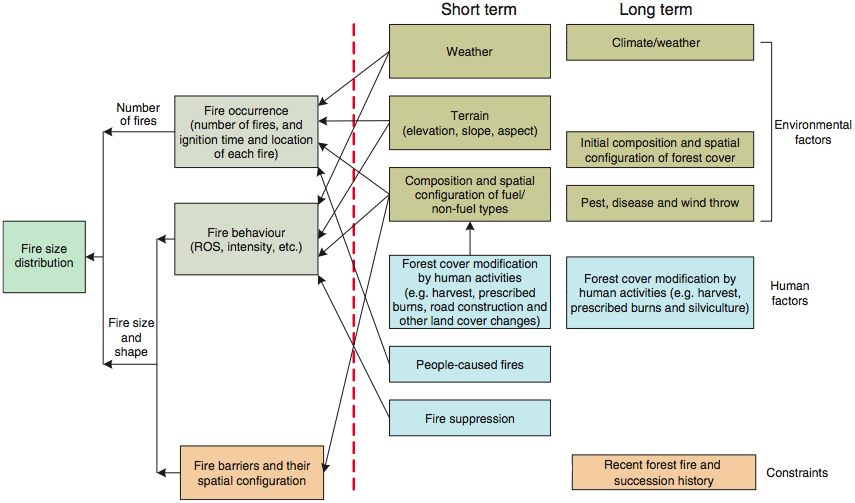
\includegraphics[width=1\textwidth]{media/fig1}
      \caption[Major causal factors of fire size distributions]{\emph{The major causal factors of forest fire size distributions (adapted from Cui and Perera 2008:239).}}
        \label{fig1}
\end{figure}

\noindent Outside of Ontario, research has shown fire suppression reducing both the number and frequency of large fires, examples include British Columbia (Hawkes \emph{et al}. 1997), Alberta (Cumming 2005), and Italy (Telesca \emph{et al}. 2005). However, other research, again in Alberta (Cumming 2000), but also in Yellowstone National Park (DiBari 2003) shows quite the opposite, in that fire suppression has resulted in fires larger than normal. The explanation offered for these rather counterintuitive results, is that the suppression of individual fires leaves behind fuel that would have normally burned. So that over the course of many years, forests protected from the natural fire cycle, become ever more dense, thereby, becoming prone to catastrophic large fires due to the accumulated build--up of fuel (Flannigan \emph{et al}. 2009). \\

\noindent The extent to which human action influences fire size distributions has therefore, significant implications for the future of commercial timber extraction in Ontario, and for the forest managers and policy makers in Ontario's Ministry of Natural Resources, who are tasked with determining the most sustainable harvest levels (Bridge \emph{et al}. 2005:41). Predictions generated from fire size distribution research have been used before, in both fire management planning, and in the development of future fire suppression policy (Minnich 1983; Minnich and Chou 1997).

\subsubsection{Fire Management Planning}
Fire managers must contend with considerable uncertainty when attempting to deploy fire suppression resources where they will be most effective (Martell \emph{et al}. 1999:135). However, historical fire size distribution data could be used to develop estimates of future fire behaviour, thereby helping fire managers make more informed decisions (Cui and Perera 2008:240). In addition, fire size distributions, within a specific fire management zone, can be combined with readily available information on the cost of suppressing fires in each class size, to estimate the cost of continued fire suppression (Cumming 2000; Calkin \emph{et al}. 2005; Donovan and Noordijk 2005).

\subsubsection{Developing Fire Suppression Policy}
Changing fire size distributions can be used as an indicator of how a forest's fire regime may be changing over time (Cui and Perera 2008:241). Correlating these changes with differing fire suppression strategies can be used to evaluate the effectiveness of fire suppression policies (Ward and Tithecott 1993; Ward \emph{et al}. 2001; Bridge \emph{et al}. 2005). Furthermore, historical fire size distribution data can be used to predict the probability of large fire events, thereby helping policy makers develop adequate disaster preparedness plans (Malamud \emph{et al}. 1998; Song \emph{et al}. 2001).

\subsection{Limitations of Fire Size Distributions}
While it is clear that fire size distributions have many applications in fire suppression research, a certain amount of caution is needed. Fire size distributions are highly specific in both spatial and temporal frames (Cui and Perera 2008:241). As such, they must not be treated as universal constants, and may not be applicable in all areas.

\subsubsection{Spatially Explicit}
Given that fire size distributions are affected by a highly complex set of causal factors (see \emph{Figure~\ref{fig1}}, on page~\pageref{fig1}), the probability estimates are likely to be highly specific to the particular area from where they were derived. This means that fire size distributions from one forest, climate or fire management zone can not be extrapolated elsewhere, without further calculations (Cui and Perera 2008:241).

\subsubsection{Scale Explicit}
Furthermore, probability estimates are specific to the particular scale and resolution of the observations from which they were derived. Therefore, estimates derived from only a few months of data for example, can not be used to predict effects happening over decades, and vice versa (Cui and Perera 2008:241).

\subsection{Forest Fire Management in Ontario}
In Canada, provincial governments are responsible for fire--suppression activities, and in Ontario, these activities are organized by the Aviation Flood and Fire Management Branch (AFFMB) of Ontario's Ministry of Natural Resources (OMNR 1997). Ontario's Ministry of Natural Resources expends a great deal of effort and resources suppressing wildfires, particularly in those areas where commercial timber harvesting is in operation (Cumming 2005:772). These resources include over 200 permanent staff, 600 seasonal firefighters, a fleet of amphibious air--tankers, helicopters and fire detection aircraft. Additional firefighting  resources are also contracted in from the private sector during periods of high activity (Martell \emph{et al}. 1999:132). \\

\noindent Fire managers assume these efforts to be effective, given that data from Ontario showed fire suppression had significantly reduced the annual area burned by wildfires over recent decades (Ward and Tithecott 1993). Some calculations suggest that the Ministry's fire suppression activities save up to 35\% of the province's annual timber harvest from being burned each year (OMNR 1997). \\

\noindent However, not all forests in Ontario are managed in the same way. Rather, the province is divided into several fire management zones (OMNR 1997), with each zone offering a different level of protection (Bridge \emph{et al}. 2005:41). These areas are classified as the Intensive, Measured, and Extensive fire management zones (see \emph{Figure~\ref{fig2}}). \\

\begin{figure}[h!]
  \centering
    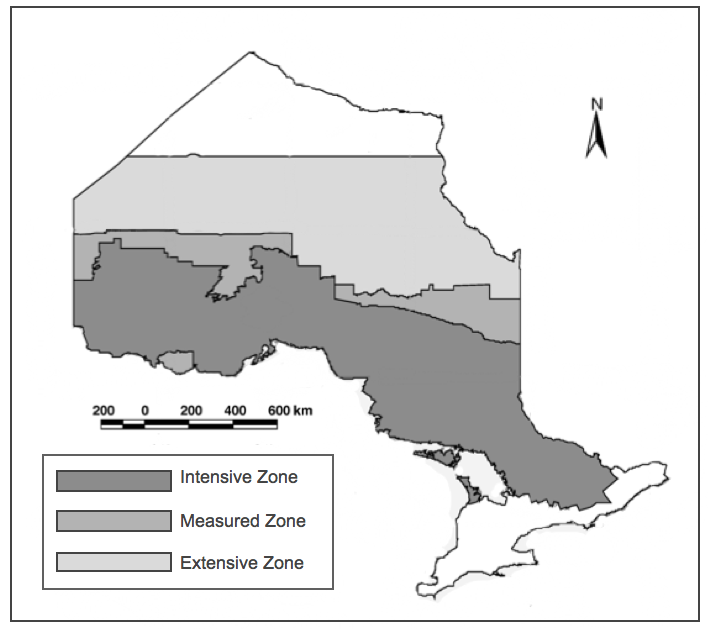
\includegraphics[width=0.7\textwidth]{media/fig2}
      \caption[Distribution of fire management zones in Ontario]{\emph{Approximate distribution of the fire management zones in the province of Ontario (adapted from Bridge \emph{et al}. 2005:41).}}
        \label{fig2}
\end{figure}

\subsubsection{Intensive Zone}
The intensive protection zone covers areas of significant commercial timber production, as well as those areas in which forest fires threaten residential housing (Bridge \emph{et al}. 2005:42). The strategy employed in the Intensive zone, therefore, is designed to minimise the damage done by forest fires by aggressively attacking all fires in the region until they are fully extinguished. At first, this action, called 'Initial Attack', involves dispatching small crews of firefighters to halt the initial spread of a new fire (Merrill and Alexander 1987). However, if a fire fails to be extinguished while small, the fire is said to have 'escaped' initial attack (Cumming 2005:773). After this point, fire fighters move to a different strategy (hereinafter referred to as \emph{Continued Suppression}), designed to manage and ultimately suppress these larger 'campaign' fires.

\subsubsection{Measured Zone}
The areas covered by the Measured zone also include commercial timber production, however these areas are considered of lesser value that those in the Intensive zone (Bridge \emph{et al}. 2005:42). For this reason, while all new fires are aggressively attacked, those fires that escape are assessed on a cost--benefit analysis (i.e., the cost of fire--fighting verses the value of the area at risk), as to whether fire suppression should continue (Hirsch \emph{et al}. 1998).

\subsubsection{Extensive Zone}
The Extensive zone covers the most northern reaches of the provence. Only when lives or property are at risk, is fire suppression employed in this region.

\subsubsection{Preventive Measures}
\noindent In addition to the activities outline above, the Ministry also employs a range of preventive measures (Martell 2001). These include, the use of prescribed burning for silvicultural management (Martell \emph{et al}. 1999:133), and educational programmes in fire safety, such as the Woods Modifications Guide, for those companies operating in forested areas (OMNR 1989).


\end{spacing}
\clearpage
